\documentclass[dvipdfmx]{beamer}
\usepackage{mySld}

\begin{document}
\title[OS]{オペレーティングシステム\\第5章 プロセス同期}
\date{}

\begin{frame}
  \titlepage
\end{frame}

%\begin{frame}
%  \frametitle
%  \tableofcontents
%\end{frame}

\section{競合(Race Condition,Competition)}
\begin{frame}
  \frametitle{共有資源}
  \begin{itemize}
    \item スレッド間の共有変数
    \item プロセス間の共有メモリ
    \item カーネル内のデータ構造
    \item ファイル
    \item 入出力装置
    \item その他
  \end{itemize}
\end{frame}

\begin{frame}
  \frametitle{競合(Race Condition,Competition)}
  \lstinputlisting{Lst/race.txt}
\end{frame}

\section{クリティカルセクション(Critical Section)}
\begin{frame}
  \frametitle{クリティカルセクション(Critical Section)}
  同時に複数のプロセス(スレッド)が実行すると競合が発生する部分\\
  (クリティカルリージョン(Critical Region)とも呼ぶ)
  \begin{enumerate}
  \item 二つ以上のプロセス(スレッド)が同時にクリティカルセクションに入らない.
  \item クリティカルセクションに入っているプロセス(スレッド)がない時は,
    待たされることなくクリティカルセクションに入ることができる.
  \item クリティカルセクションに入るために永遠に待たされることがない.
  \end{enumerate}
\end{frame}

\section{相互排他(mutual exclusion)}
\begin{frame}
  \frametitle{相互排他(mutual exclusion)}
  \begin{itemize}
  \item エントリーセクション(Entry Section)\\
    クリティカルセクションに入る手続き
  \item エグジットセクション(Exit Section)\\
    クリティカルセクションを出る手続き
  \end{itemize}
\end{frame}

\begin{frame}
  \frametitle{割込み禁止}
  \lstinputlisting{Lst/disableInterrupt.txt}
  \begin{itemize}
  \item エントリーセクション(Entry Section)\\
    割り込み禁止の場合はDI命令
  \item エグジットセクション(Exit Section)\\
    割り込み禁止の場合はEI命令
  \end{itemize}
\end{frame}

\begin{frame}
  \frametitle{ハードウェア構成}
  \fig{scale=0.41}{hardBlock-crop.pdf}
  \begin{itemize}
    \item SMP(Symmetric Multiprocessing)
    \item CPUはメモリを共有する
  \end{itemize}
\end{frame}

\begin{frame}
  \frametitle{専用命令(TS命令)}
  TS(Test and Set)命令はSMPシステムでの相互排除に使用できる.\\
  「TS  R, M」は以下を{\bf アトミック(atomic)}に実行する.
  \begin{enumerate}
  \item バスをロックする
  \item $R \leftarrow [M]$
  \item {\tt if (R==0) } $z \leftarrow 1$ {\tt else} $z \leftarrow 0$
  \item $[M] \leftarrow 1$
  \item バスのロックを解除する
  \end{enumerate}
\end{frame}

\begin{frame}
  \frametitle{専用命令(TS命令の使用例)}
  \lstinputlisting{Lst/testAndSet.s}
\end{frame}

\begin{frame}
  \frametitle{専用命令(SW命令)}
  SW(Swap)命令もSMPシステムでの相互排除に使用できる.\\
  「SW  R, M」は以下を{\bf アトミック(atomic)}に実行する.
  \begin{enumerate}
  \item バスをロックする
  \item $T \leftarrow [M]$
  \item $[M] \leftarrow R$
  \item $R \leftarrow T$
  \item バスのロックを解除する
  \end{enumerate}
  ここで $T$ はCPU内部の一時的なレジスタ\\
  ($T$ レジスタの存在はプログラムから見えない)
\end{frame}

\begin{frame}
  \frametitle{専用命令(SW命令の使用例)}
  \lstinputlisting{Lst/swap.s}
\end{frame}

\begin{frame}
  \frametitle{専用命令(CAS命令)}
  CAS(Compare And Swap)命令もSMPシステムでの相互排除に使用できる.
  「CAS  R0, R1, M」は,以下を{\bf アトミック(atomic)}に実行する.
  \begin{enumerate}
  \item バスをロックする
  \item $T \leftarrow [M]$
  \item {\tt if ($T==R0$) \{} $[M] \leftarrow R1;~ z \leftarrow 1;$
    {\tt \} else \{} $R0 \leftarrow T;~  z \leftarrow 0;$ {\tt \}}
  \item バスのロックを解除する
  \end{enumerate}
  \vspace{1em}
  \lstinputlisting{Lst/cas.txt}
  {\bf ロックフリー(Lock-free)}なアルゴリズム
\end{frame}

\begin{frame}
  \frametitle{Peterson のアルゴリズム}
  \lstinputlisting{Lst/peterson.txt}
\end{frame}

\section{セマフォ(Semaphore)}
\begin{frame}
  \frametitle{セマフォ(Semaphore)}
  1965年に E. W. Dijkstra が提案したデータ型である.
  \begin{itemize}
  \item {\bf ビジーウェイティング(Busy Waiting)}を用いない
  \item オペレーティングシステムが提供する洗練された同期機構
  \item システムコール等でユーザプロセスに提供
  \item サブルーチンとしてサービスモジュール等に提供
  \end{itemize}

{\bf セマフォ(Semaphore:腕木式信号機)}の元々の意味はこれ!

\begin{center}

\includegraphics[scale=0.4]{Fig/semaphore.png}
\end{center}
\end{frame}

\begin{frame}
  \frametitle{セマフォ(Semaphore)}
  \begin{itemize}
  \item セマフォはデータ構造({\color{red} セマフォ型},セマフォ構造体)
  \item カウンタは0以上の整数値(0は{\color{red} 赤信号}の意味)
  \item プロセスの待ち行列を作ることができる.
  \item セマフォ型の変数に{\bf P操作}と{\bf V操作}ができる.
  \item {\bf P操作({\it Proberen}:try)}
  \item {\bf V操作({\it Verhogen}:raise)}
  \item ユーザプロセスには{\bf P,Vシステムコール}が提供される
  \item サービスモジュールやデバイスドライバには{\bf P,Vサブルーチン}
  \end{itemize}

セマフォはプロセス(スレッド)の状態を{\bf 待ち(Waiting)状態}に変える.
{\bf ビジーウェイティング(Busy Waiting)では無い}のでCPUを無駄遣いすることはない.
\end{frame}

\begin{frame}
  \frametitle{セマフォ(Semaphore)のP操作}
  {\bf P操作(P(S))}
  \begin{enumerate}
  \item セマフォ(S)の値が1以上ならセマフォの値を1減らす.
  \item 値が0ならプロセス(スレッド)を待ち(Waiting)状態にし,
  \item セマフォの待ち行列に追加する.
  \end{enumerate}
  クリティカルセクションのエントリーセクション等で使用できる.

  \begin{center}
    \begin{minipage}{0.6\columnwidth}
      \lstinputlisting{Lst/semP.c}
    \end{minipage}
  \end{center}
\end{frame}

\begin{frame}
  \frametitle{セマフォ(Semaphore)のV操作}
  {\bf V操作(V(S))}
  \begin{enumerate}
  \item 待っているプロセス(スレッド)が無い場合は,セマフォ(S)の値を1増やす.
  \item セマフォ(S)の待ち行列にプロセス(スレッド)がある場合は,
    それらの一つを起床させる.
  \end{enumerate}
  クリティカルセクションのエグジットセクション等で使用できる.

  \begin{center}
    \begin{minipage}{0.6\columnwidth}
      \lstinputlisting{Lst/semV.c}
    \end{minipage}
  \end{center}
\end{frame}

\begin{frame}
  \frametitle{セマフォの使用例(相互排除問題)}
  \lstinputlisting{Lst/semMutex.c}
  {\bf 初期値が1のセマフォを用いる.}
\end{frame}

\begin{frame}
  \frametitle{セマフォの使用例(生産者・消費者問題)}
  \lstinputlisting{Lst/semProducerConsumer.c}
\end{frame}

\begin{frame}
  \frametitle{セマフォの使用例(複数生産者・複数消費者問題 1/2)}
  \lstinputlisting{Lst/semMultiProducerConsumer1.c}
\end{frame}

\begin{frame}
  \frametitle{セマフォの使用例(複数生産者・複数消費者問題 2/2)}
  \lstinputlisting{Lst/semMultiProducerConsumer2.c}
\end{frame}

\begin{frame}
  \frametitle{セマフォの使用例(リーダ・ライタ問題 1/2)}
  \lstinputlisting{Lst/semReaderWriter1.c}
  {\bf 排他ロック(exclusive lock)}
\end{frame}

\begin{frame}
  \frametitle{セマフォの使用例(リーダ・ライタ問題 2/2)}
  \lstinputlisting{Lst/semReaderWriter2.c}
  {\bf 共有ロック(shared lock)}
\end{frame}

\section{TacOSのセマフォ}
\begin{frame}
  \frametitle{TacOSのセマフォ構造体(カーネル内)}
  \lstinputlisting{Lst/sem.hmm}
  \begin{itemize}
    \item セマフォは最大30個(TaCのメモリは小さい)
    \item セマフォ構造体の名前は{\tt Sem}
    \item {\tt cnt}がセマフォの値(0以上)
    \item {\tt queue}に,
      このセマフォを待っているプロセスの待ち行列を作る.
  \end{itemize}
\end{frame}

\begin{frame}
  \frametitle{TacOSのセマフォ関連データ構造(カーネル内)}
  \begin{center}
    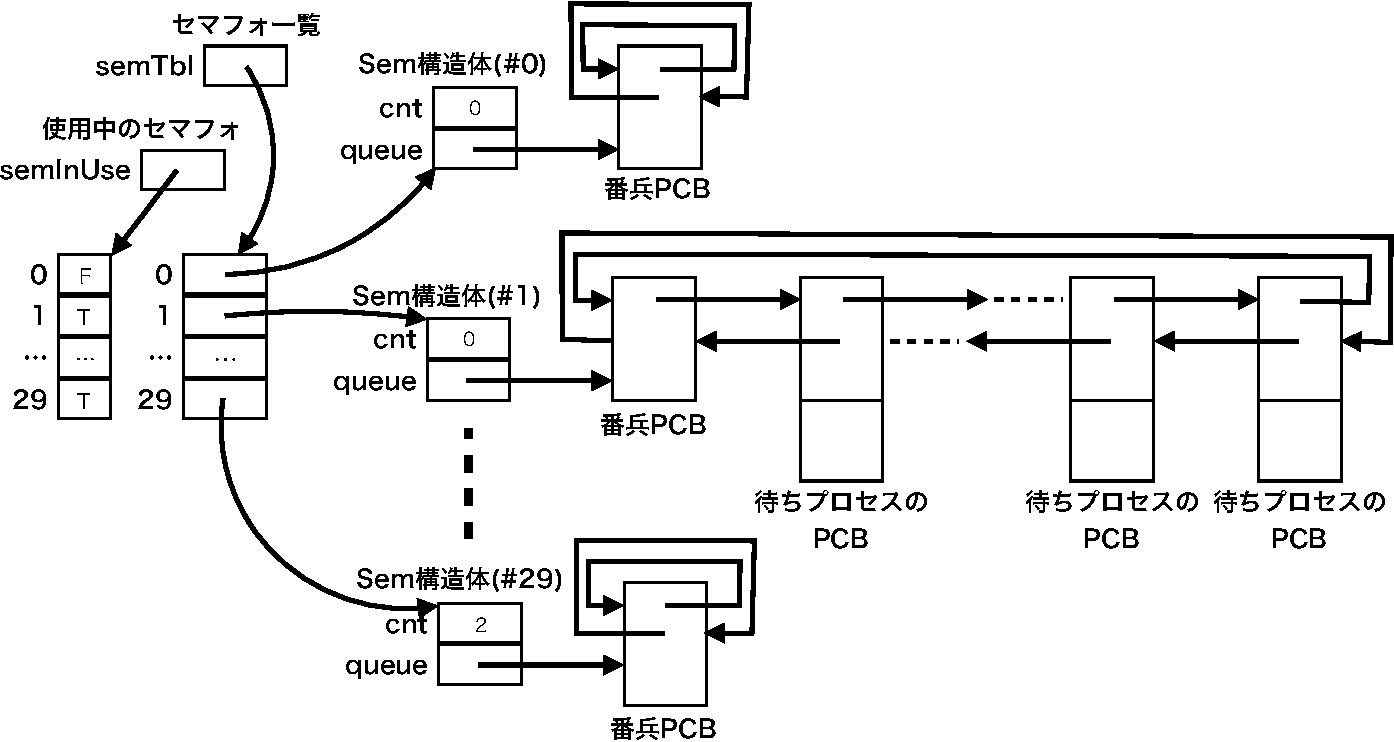
\includegraphics[scale=0.45]{Fig/tacosSemaphore-crop.pdf}
  \end{center}
  \begin{itemize}
    \item TacOSでは,セマフォを{\tt semTbl}のインデクスで識別する.
    \item Sem構造体(\#0,\#1,\#29)は,未使用,待ちあり,待ちなしの例
  \end{itemize}
\end{frame}

\begin{frame}
  \frametitle{TacOSでのセマフォの架空の使用例}
  \lstinputlisting{Lst/tacosSemUse.cmm}
\end{frame}

\begin{frame}
  \frametitle{TacOSのセマフォ割当て解放ルーチン(カーネル内)}
  \lstinputlisting{Lst/tacosNewSem.cmm}
\end{frame}

\begin{frame}
  \frametitle{TacOSのP操作ルーチン(カーネル内)}
  \lstinputlisting{Lst/tacosSemP.cmm}
\end{frame}

\begin{frame}
  \frametitle{TacOSのV操作ルーチン(1/2)(カーネル内)}
  \lstinputlisting{Lst/tacosSemV1.cmm}
  \begin{itemize}
  \item {\tt iSemV()}は割込禁止で呼び出す.
  \end{itemize}
\end{frame}

\begin{frame}
  \frametitle{TacOSのV操作ルーチン(2/2)(カーネル内)}
  \lstinputlisting{Lst/tacosSemV2.cmm}
  \begin{itemize}
  \item {\tt iSemV()}を呼び出す前に割込禁止にする.
  \item {\tt iSemV()}がtrueで返ったらプロセスの切換えを試みる.
  \item {\tt yield()}でプリエンプションしたプロセスは,
    {\tt yield()}から実行が再開される.
  \end{itemize}
\end{frame}

\begin{frame}
  \frametitle{TacOSのCPUフラグ操作関数(カーネル内)}
  \lstinputlisting{Lst/setPri.s}
  \begin{itemize}
  \item CPUのPSWのフラグに割込禁止ビットがある.
  \item {\tt C--}言語から{\tt setPri()}関数として呼び出せるようにするには,
    アセンブリ言語プログラムで{\tt \_setPri}ラベルを宣言する必要がある.
  \item {\tt C--}言語プログラムは引数をスタックに積んで関数をCALLする.
  \item アセンブリ言語プログラムで引数を参照するには,
    ({\tt SP}相対で)スタックから取り出す.
    ({\tt SP+0}番地が{\tt PC},{\tt SP+2}番地が第1引数)
  \item 関数の返り値は,{\tt G0}レジスタに入れて返す.
  \item {\tt reti}命令はスタックからフラグとPCを一度に取り出す.
  \end{itemize}
\end{frame}

\end{document}
